\documentclass{article}

\usepackage{fancyhdr}
\usepackage{extramarks}
\usepackage{amsmath}
\usepackage{amsthm}
\usepackage{amsfonts}
\usepackage{amssymb}
\usepackage{graphicx}
\usepackage{caption,subcaption}
\usepackage{subfig}
\usepackage{enumerate}          % For enumerates indexed by letters
\usepackage{bm}                 % For bold letters
\usepackage{algorithm2e}        % For pseudocode

%
% Basic Document Settings
%

\topmargin=-0.45in
\evensidemargin=0in
\oddsidemargin=0in
\textwidth=6.5in
\textheight=9.0in
\headsep=0.25in

\linespread{1.1}

\pagestyle{fancy}
\lhead{\hmwkAuthorName}
\chead{\hmwkClass:\ \hmwkTitle}
\rhead{\firstxmark}
\lfoot{\lastxmark}
\cfoot{\thepage}

\renewcommand\headrulewidth{0.4pt}
\renewcommand\footrulewidth{0.4pt}

\setlength\parindent{0pt}

\setcounter{section}{-1}




%
% Homework Details
%   - Title
%   - Due date
%   - Class
%   - Section/Time
%   - Instructor
%   - Author
%

\newcommand{\hmwkTitle}{Homework 3}
\newcommand{\hmwkDueDate}{November 23, 2016}
\newcommand{\hmwkClass}{CSE 546}
\newcommand{\hmwkAuthorName}{Brian de Silva}

%
% Title Page
%

\title{
    \vspace{2in}
    \textmd{\textbf{\hmwkClass:\ \hmwkTitle}}\\
    \normalsize\vspace{0.1in}\small{Due\ on\ \hmwkDueDate\ }\\
    \vspace{3in}
}

\author{\textbf{\hmwkAuthorName}}
\date{}


% Useful commands
\newcommand{\E}{\mathbb{E}}
\newcommand{\Var}{\mathrm{Var}}
\newcommand{\Cov}{\mathrm{Cov}}
\newcommand{\Bias}{\mathrm{Bias}}
\newcommand{\bbm}{\begin{bmatrix}}
\newcommand{\ebm}{\end{bmatrix}}
\newcommand{\R}{\mathbb{R}}
\newcommand{\y}{\hat \bm{y}}
\newcommand{\yi}{\hat \bm{y_i}}
\newcommand{\X}{\bm{X}}
\newcommand{\w}{\bm{w}}
\newcommand{\T}{\mathcal{T}}
\newcommand{\Tr}{\mathrm{Tr}}


\begin{document}

\maketitle

\pagebreak

% Problem 0
\section{Collaborators and Acknowledgements}
I collaborated with Kelsey Maass on problem two.

% Problem 1
\section{PCA and reconstruction}
\subsection{Matrix Algebra Review}
\begin{enumerate}
	\item Recall that for $A\in\R^{n\times d}$ and $C\in\R^{d\times n}$, $(AC)_{ij} = \sum^d_{k=1}a_{ik}c_{kj}$. Also, $(B^T)_{ij} = B_{ji}$. Hence
	\[
		(AB^T)_{ij} = \sum^d_{i=1}(A)_{ik}(B^T)_{jk} = \sum^d_{i=1}a_{ik}b_{kj}.
	\]

	Plugging this into the definition of the trace gives
	\begin{align*}
		\Tr(AB^T) &= \sum^n_{i=1}\left(\sum^d_{k=1}(AB^T)_{ii}\right)\\
		&= \sum^n_{i=1}\left(\sum^d_{k=1}a_{ik}b_{ik}\right).
	\end{align*}
	Similarly,
	\[
		(B^TA)_{ij} = \sum^{n}_{k=1}b_{ki}a_{kj}
	\]
	and, by switching the order of addition,
	\begin{align*}
		\Tr(B^TA) &= \sum^d_{i=1}\left(B^TA\right)_{ii}\\
		&= \sum^d_{i=1}\left(\sum^n_{k=1}b_{ki}a_{ki} \right) \\
		&= \sum^n_{i=1}\left(\sum^d_{k=1}b_{ki}a_{ki} \right) \\
		&= \Tr(AB^T).
	\end{align*}

	\item The outer equality follows from the definition of the trace:
	\begin{align*}
		\Tr(\Sigma) = \Tr\left(\tfrac1nX^TX\right) = \frac1n\sum^d_{i=1}(X^TX)_{ii} &= \frac1n \sum^d_{i=1}\left( \sum^n_{k=1}x_{ik}^2 \right)\\
		&= \frac1n\sum^d_{i=1}\|X_i\|^2.
	\end{align*}
	For the other equality, we need some standard linear algebra results. Since $\Sigma$ is symmetric and real, it has a real orthogonal eigendecomposition. That is to say, there exists an orthogonal matrix $Q$ and a diagonal matrix $\Lambda$ with diagonal entries $\lambda_1,\lambda_2,\dots,\lambda_d$ such that
	\[
		\Sigma = Q\Lambda Q^T.
	\]
	Using our result from part 1, we have
	\[
		\Tr(\Sigma) = \Tr\left(Q\Lambda Q^T\right) = \Tr\left((Q\Lambda) Q^T\right) = \Tr\left(Q^TQ\Lambda\right) = \Tr(\Lambda) = \sum^d_{i=1}\lambda_i.
	\]
\end{enumerate}

\subsection{PCA}
\begin{enumerate}
	\item Without centering the data, the eigenvalues we obtain for $\Sigma$ are 
	\begin{align*}
		\lambda_1 &= 2476871.877922\\
		\lambda_2 &= 285468.253236\\
		\lambda_{10} &= 81022.153964\\
		\lambda_{30} &= 23690.383772\\
		\lambda_{50} &= 11076.827129.
	\end{align*}
	The sum of the eigenvalues is $\sum^{784}_{i=1}\lambda_i = 5709846.669117$. Notice that the first eigenvalue accounts for almost half of the total of all the eigenvalues.
	\item
	\begin{figure}
        \centering
        \includegraphics[width=.85\textwidth]{fre1}
        \caption{Fractional reconstruction error using the top 1 through 50 principal components} 
        \label{fig:fre1}
    \end{figure}
	We plot the fractional reconstruction error retaining 1 through 50 of the top principal directions in Figure \ref{fig:fre1}.
	\item The first eigenvector captures the average image of the dataset. The first eigenvalue gives some indication of how close the images are to this average one. All of the images have a large amount of blank space in common, and so they are, in a sense, well-approximated by the average image. This explains why the first eigenvalue is so large compared to the rest.
	\item 
	\begin{figure}
        \centering
        \includegraphics[width=.85\textwidth]{fre2}
        \caption{Fractional reconstruction error using the top 2 through 50 principal components} 
        \label{fig:fre2}
    \end{figure}
    We show the fractional reconstruction error for dimensions 2 through 50 in Figure \ref{fig:fre2}.
\end{enumerate}

\subsection{Visualization of the Eigen-Directions}
\begin{enumerate}
	\item
	\begin{figure}
        \centering
        \includegraphics[width=.95\textwidth]{topEvs}
        \caption{The eigenvectors corresponding to the 10 largest eigenvalues of $\Sigma$. Grey corresponds to values of 0, black to positive values, and white to negative values.} 
        \label{fig:topEvs}
    \end{figure}
	Visualizations of the top 10 eigenvectors are shown in Figure \ref{fig:topEvs}.
	\item As I mentioned in a previous problem, the first eigenvector captures the average of all the images. The other eigenvalues appear to contain information about patterns encountered in many of the digits. The second eigenvalue, for example, appears to encapsulate the roundness that many digits exhibit (i.e. 0,3,6,8, and 9). 
\end{enumerate}

\subsection{Visualization and Reconstruction}
\begin{enumerate}
	\item 
	\begin{figure}
        \centering
        \includegraphics[width=.95\textwidth]{digits}
        \caption{Five different images from the MNIST dataset} 
        \label{fig:digits}
    \end{figure}
    Figure \ref{fig:digits} shows five images from the MNIST dataset (the first five, in fact).
    \item 
    \begin{figure}
        \centering
        \begin{subfigure}[b]{0.95\textwidth}
        	\centering
        	\includegraphics[width=0.7\linewidth]{02evRecon}
        	\caption{Reconstruction with two eigenvectors}
        	\label{fig:2ev}
        \end{subfigure}
        \begin{subfigure}[b]{0.95\textwidth}
        	\centering
        	\includegraphics[width=0.7\linewidth]{05evRecon}
        	\caption{Reconstruction with five eigenvectors}
        	\label{fig:4ev}
        \end{subfigure}
        \caption{Reconstruction of MNIST images using two and five eigenvectors}
        \label{fig:evRecons1}
    \end{figure}

    \begin{figure}
    	\centering
        \begin{subfigure}[b]{0.95\textwidth}
        	\centering
        	\includegraphics[width=0.7\linewidth]{10evRecon}
        	\caption{Reconstruction with 10 eigenvectors}
        	\label{fig:10ev}
        \end{subfigure}
        \begin{subfigure}[b]{0.95\textwidth}
        	\centering
        	\includegraphics[width=0.7\linewidth]{20evRecon}
        	\caption{Reconstruction with 20 eigenvectors}
        	\label{fig:20ev}
        \end{subfigure}
        \begin{subfigure}[b]{0.95\textwidth}
        	\centering
        	\includegraphics[width=0.7\linewidth]{50evRecon}
        	\caption{Reconstruction with 50 eigenvectors}
        	\label{fig:50ev}
        \end{subfigure}
        \caption{Reconstructions of MNIST images using different numbers of eigenvectors} 
        \label{fig:evRecons2}
    \end{figure}
    Figure \ref{fig:evRecons1} shows the reconstructions produced using two and five eigenvectors, respectively. Figure \ref{fig:evRecons2} visualizes the reconstructions utilizing 10, 20, and 50 eigenvectors, respectively.
    \item The two-eigenvector reconstruction is not very good. Under this projection some of the digits look almost identical. Using just five eigenvectors, one can already make out most of the digits. With 10 eigenvectors these digits become even clearer, though the 4 appears to be difficult to represent. The 20-eigenvalue approximation is crisper than the previous ones, but the increase in quality it starting to slow. Adding another 30 eigenvalues makes it very easy to discern the digits. Overall, adding more eigenvalues improves the projection quality, but the returns are diminishing.
\end{enumerate}

% ---------------------------------

% Problem 2
\section{Let's get to state of the art on MNIST!}
\subsection{Least Squares}
The code for this problem is contained in \texttt{hw3-2-1.py}.
\begin{enumerate}
	\item To obtain the results presented in this section I used the following parameters: a mini-batch size of 10, no regularization, stochastic gradient descent with a learning rate of $10^{-5} / (2\sqrt{t+1})$, where $t$ is the epoch, and initial weights all 0. I used the Fourier features with a kernel bandwidth that is 1/2 the approximate mean distance between points in the dataset. In order to approximate this distance I randomly sampled 100 pairs of points from the training data and took the mean of their Euclidean distances from one another. This parameter was on the order of $10^3$. To obtain the plots below I ran SGD for 10 epochs.


	\item
	\begin{figure}
        \centering
        \includegraphics[width=.95\textwidth]{sqlossLS10epoch}
        \caption{The square loss of Stochastic gradient descent for the least squares problem applied to Fourier features of the projected MNIST dataset as a function of iteration, starting at iteration 0} 
        \label{fig:sqlossLS10epoch}
    \end{figure}
    \begin{figure}
        \centering
        \includegraphics[width=.95\textwidth]{sqlossLS10epochtrunc}
        \caption{The square loss of Stochastic gradient descent for the least squares problem applied to Fourier features of the projected MNIST dataset as a function of iteration, starting after one epoch} 
        \label{fig:sqlossLS10epochtrunc}
    \end{figure}
	Figure \ref{fig:sqlossLS10epoch} shows the squared loss after each epoch on the training and test sets for both $w_t$ (labeled ``w'' in the legend) and the average weight vector over each epoch (denoted ``wAvg'' in the legend). To better view how the square loss is decreasing Figure \ref{fig:sqlossLS10epochtrunc} shows the same plot with one set of data points removed--those corresponding to the initial error.
	\item
    \begin{figure}
        \centering
        \includegraphics[width=.95\textwidth]{z1lossLS10epoch}
        \caption{The 0/1 loss of Stochastic gradient descent for the least squares problem applied to Fourier features of the projected MNIST dataset as a function of iteration, starting after one epoch} 
        \label{fig:z1lossLS10epoch}
    \end{figure}
	Figure \ref{fig:z1lossLS10epoch} plots the 0/1 loss on the training and test sets after each epoch for both the actual set of weights and the average weights. Note that the initial 0/1 loss (around 0.9--as good as randomly guessing the labels) has not been included in the plot. This makes it easier to see what is happening.
	\item After 10 epochs my final training squared loss was about 0.04036 and my final training 0/1 loss was 0.005100. Both of these numbers were computed using the average weights over the last epoch. The total number of misclassifications made with this weight vector was 306 (out of 60000).
	\item After 10 epochs my final square loss on the test set was 0.06111 and my final 0/1 loss on this set was 0.013900. Both of these numbers were computed using the average weights over the last epoch. The total number of misclassifications made with this weight vector was 139 (out of 10000).

\end{enumerate}

\subsection{EXTRA CREDIT: Softmax Classification}
\begin{enumerate}
	\item For the results in this section I used a learning rate of $10^{-1} / 4\sqrt{t+1}$, where $t$ is the iteration within the current epoch, and a mini-batch size of 10. I also used a regularization parameter of 1. I could not get the method to do much beyond the first epoch, even after lots of experimentation with step sizes, batch sizes, and regularization parameters. Perhaps changing the bandwidth, $\sigma$, could have improved things, but the instructions said to use the same one as before. The code for this problem is in \texttt{hw3-2-2.py}.
	\item 
	\begin{figure}
        \centering
        \includegraphics[width=.95\textwidth]{logLossSoftmax30epoch}
        \caption{The log loss of Stochastic gradient descent for the softmax classification problem applied to the Fourier features of the projected MNIST dataset as a function of iteration, starting at iteration 0}
        \label{fig:logLossSoftmax30epoch}
    \end{figure}
    Figure \ref{fig:logLossSoftmax30epoch} plots the log loss for Stochastic gradient descent applied to the log likelihood using the Fourier features. Plotted are the log losses on the training and test sets for the regular and average weight vectors.
    \item
    \begin{figure}
        \centering
        \includegraphics[width=.95\textwidth]{z1LossSoftmax30epoch}
        \caption{The 0/1 loss of Stochastic gradient descent for the softmax classification problem applied to the Fourier features of the projected MNIST dataset as a function of iteration, starting after an epoch has passed}
        \label{fig:z1LossSoftmax30epoch}
    \end{figure}
    Figure \ref{fig:z1LossSoftmax30epoch} shows the 0/1 loss on the same problem for the training and test sets, computed with both the weight vectors and the epoch-averaged weights.
    \item My final training log and 0/1 losses on this problem were 0.17606464 and 0.035783, respectively. This 0/1 loss corresponds to missing 2147 digits out of 60000.
    \item My final testing log and 0/1 losses were 0.178957 and 0.038800, respectively. This 0/1 loss corresponds to 388 misses out of 10000 trials

\end{enumerate}

\subsection{EXTRA CREDIT: Back to those random Neural Net Features}
\begin{enumerate}
	\item For the results presented in this section I used a step-size of $10^-8 / \sqrt{1+t}$, where $t$ is the iteration number within the current epoch. I used stochastic gradient descent with a batch size of 10 for optimization and used a regularization constant of 1. 18 epochs were required to get the results below. The code for this problem is in \texttt{hw3-2-3.py}.
	\item 
	\begin{figure}
        \centering
        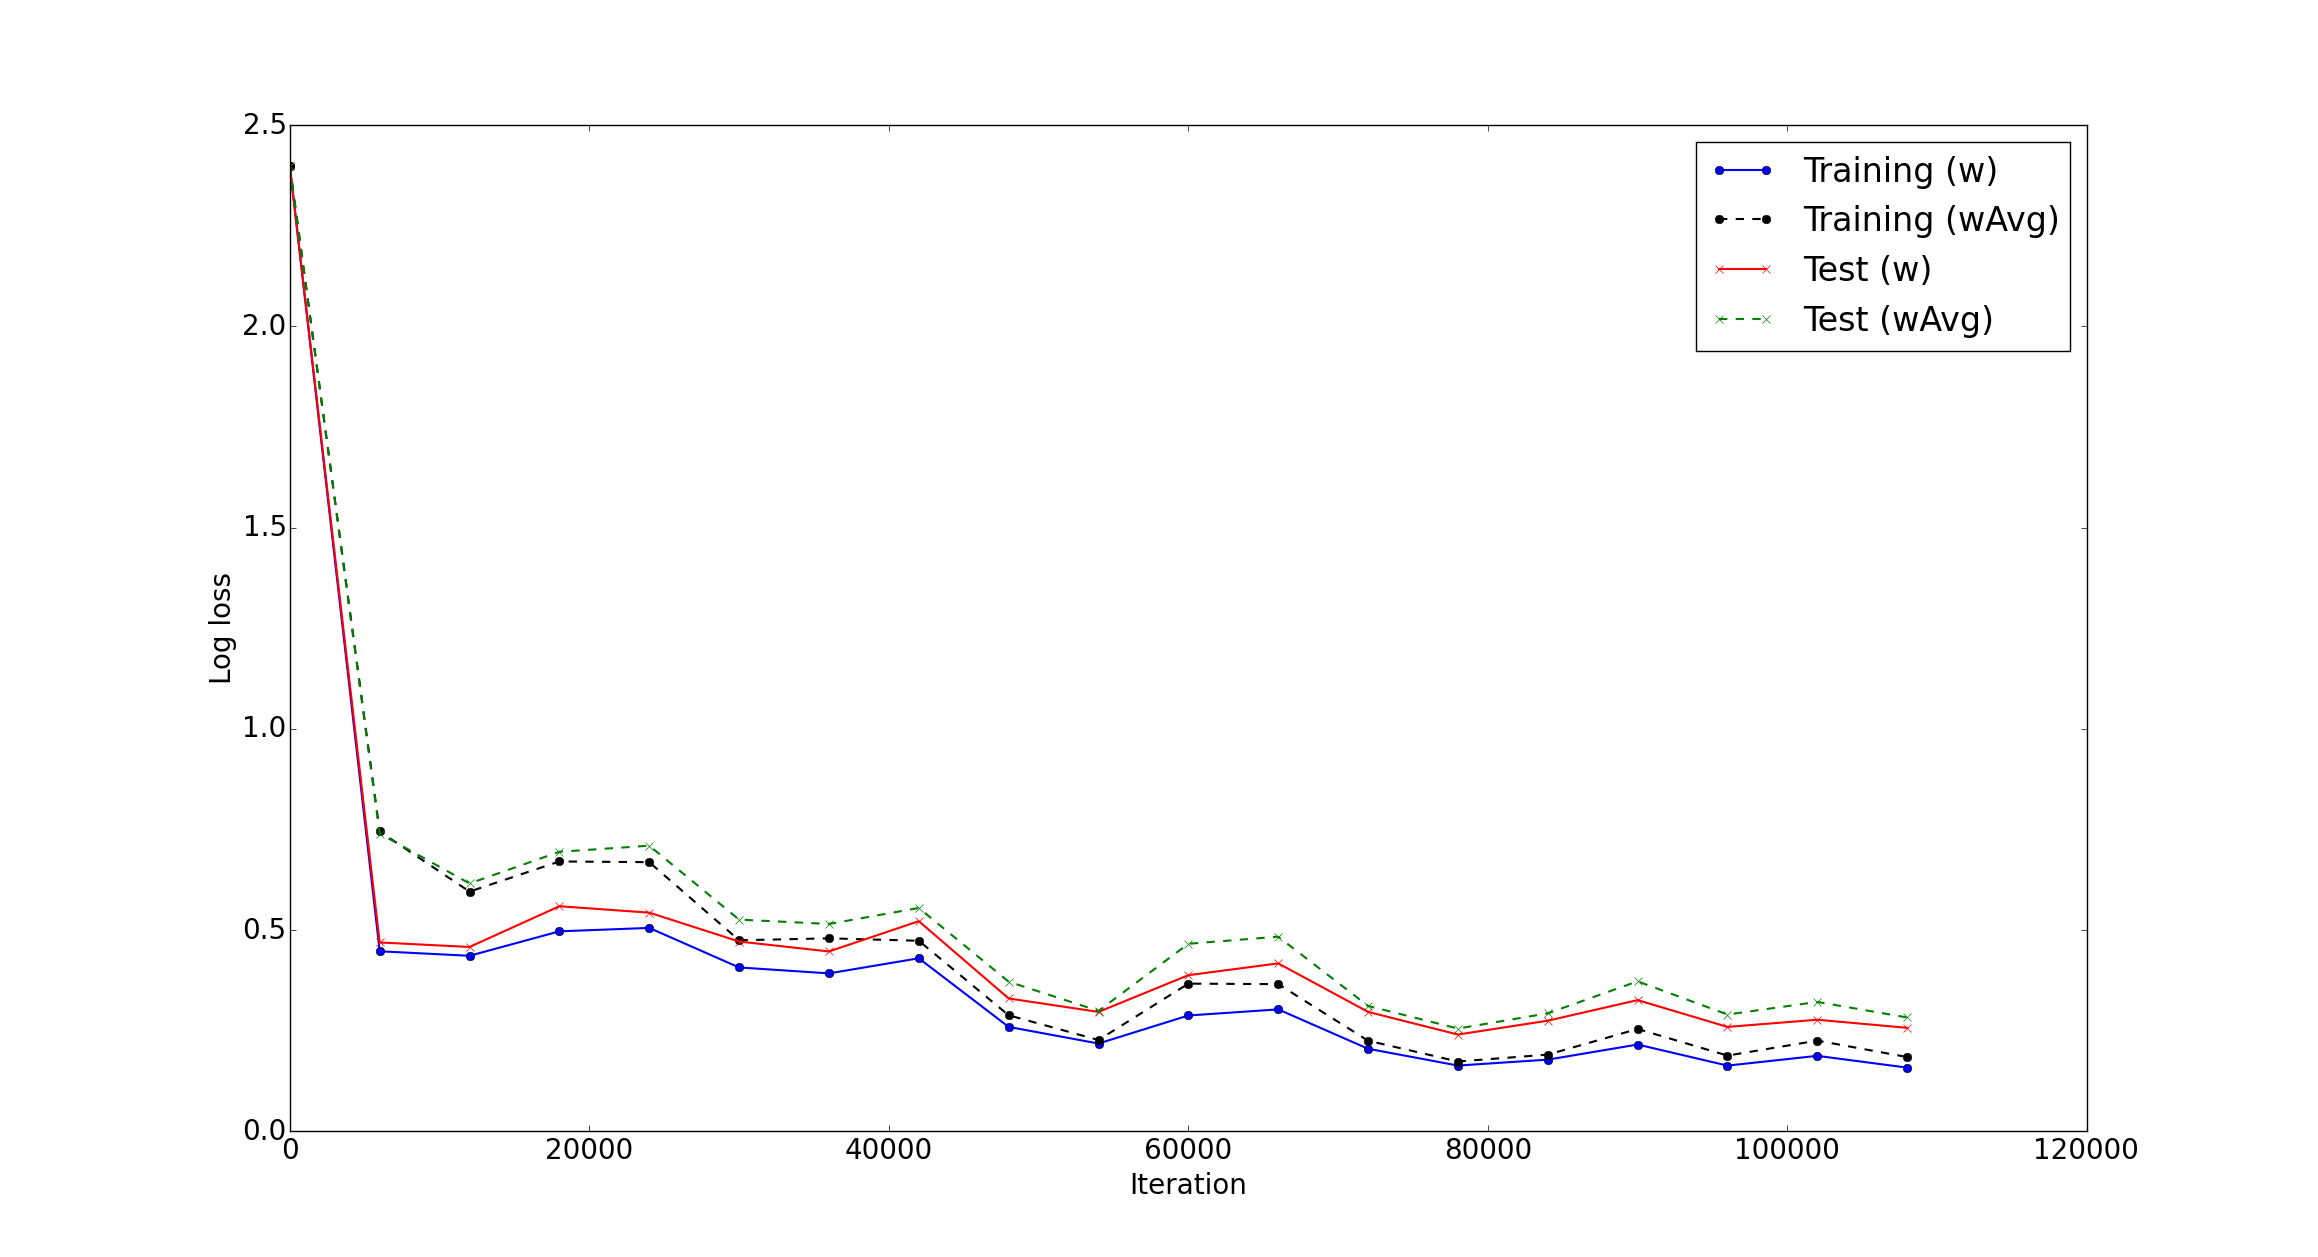
\includegraphics[width=.95\textwidth]{logLossNNFeats18Epochs}
        \caption{The log loss of Stochastic gradient descent for the softmax classification problem applied to random neural net features of the projected MNIST dataset as a function of iteration, starting at iteration 0}
        \label{fig:logLossNNFeats18Epochs}
    \end{figure}
    Figure \ref{fig:logLossNNFeats18Epochs} gives a plot of the decay of the log loss on the training and test sets, using both the actual weights and the epoch-averaged ones.
    \item 
    \begin{figure}
        \centering
        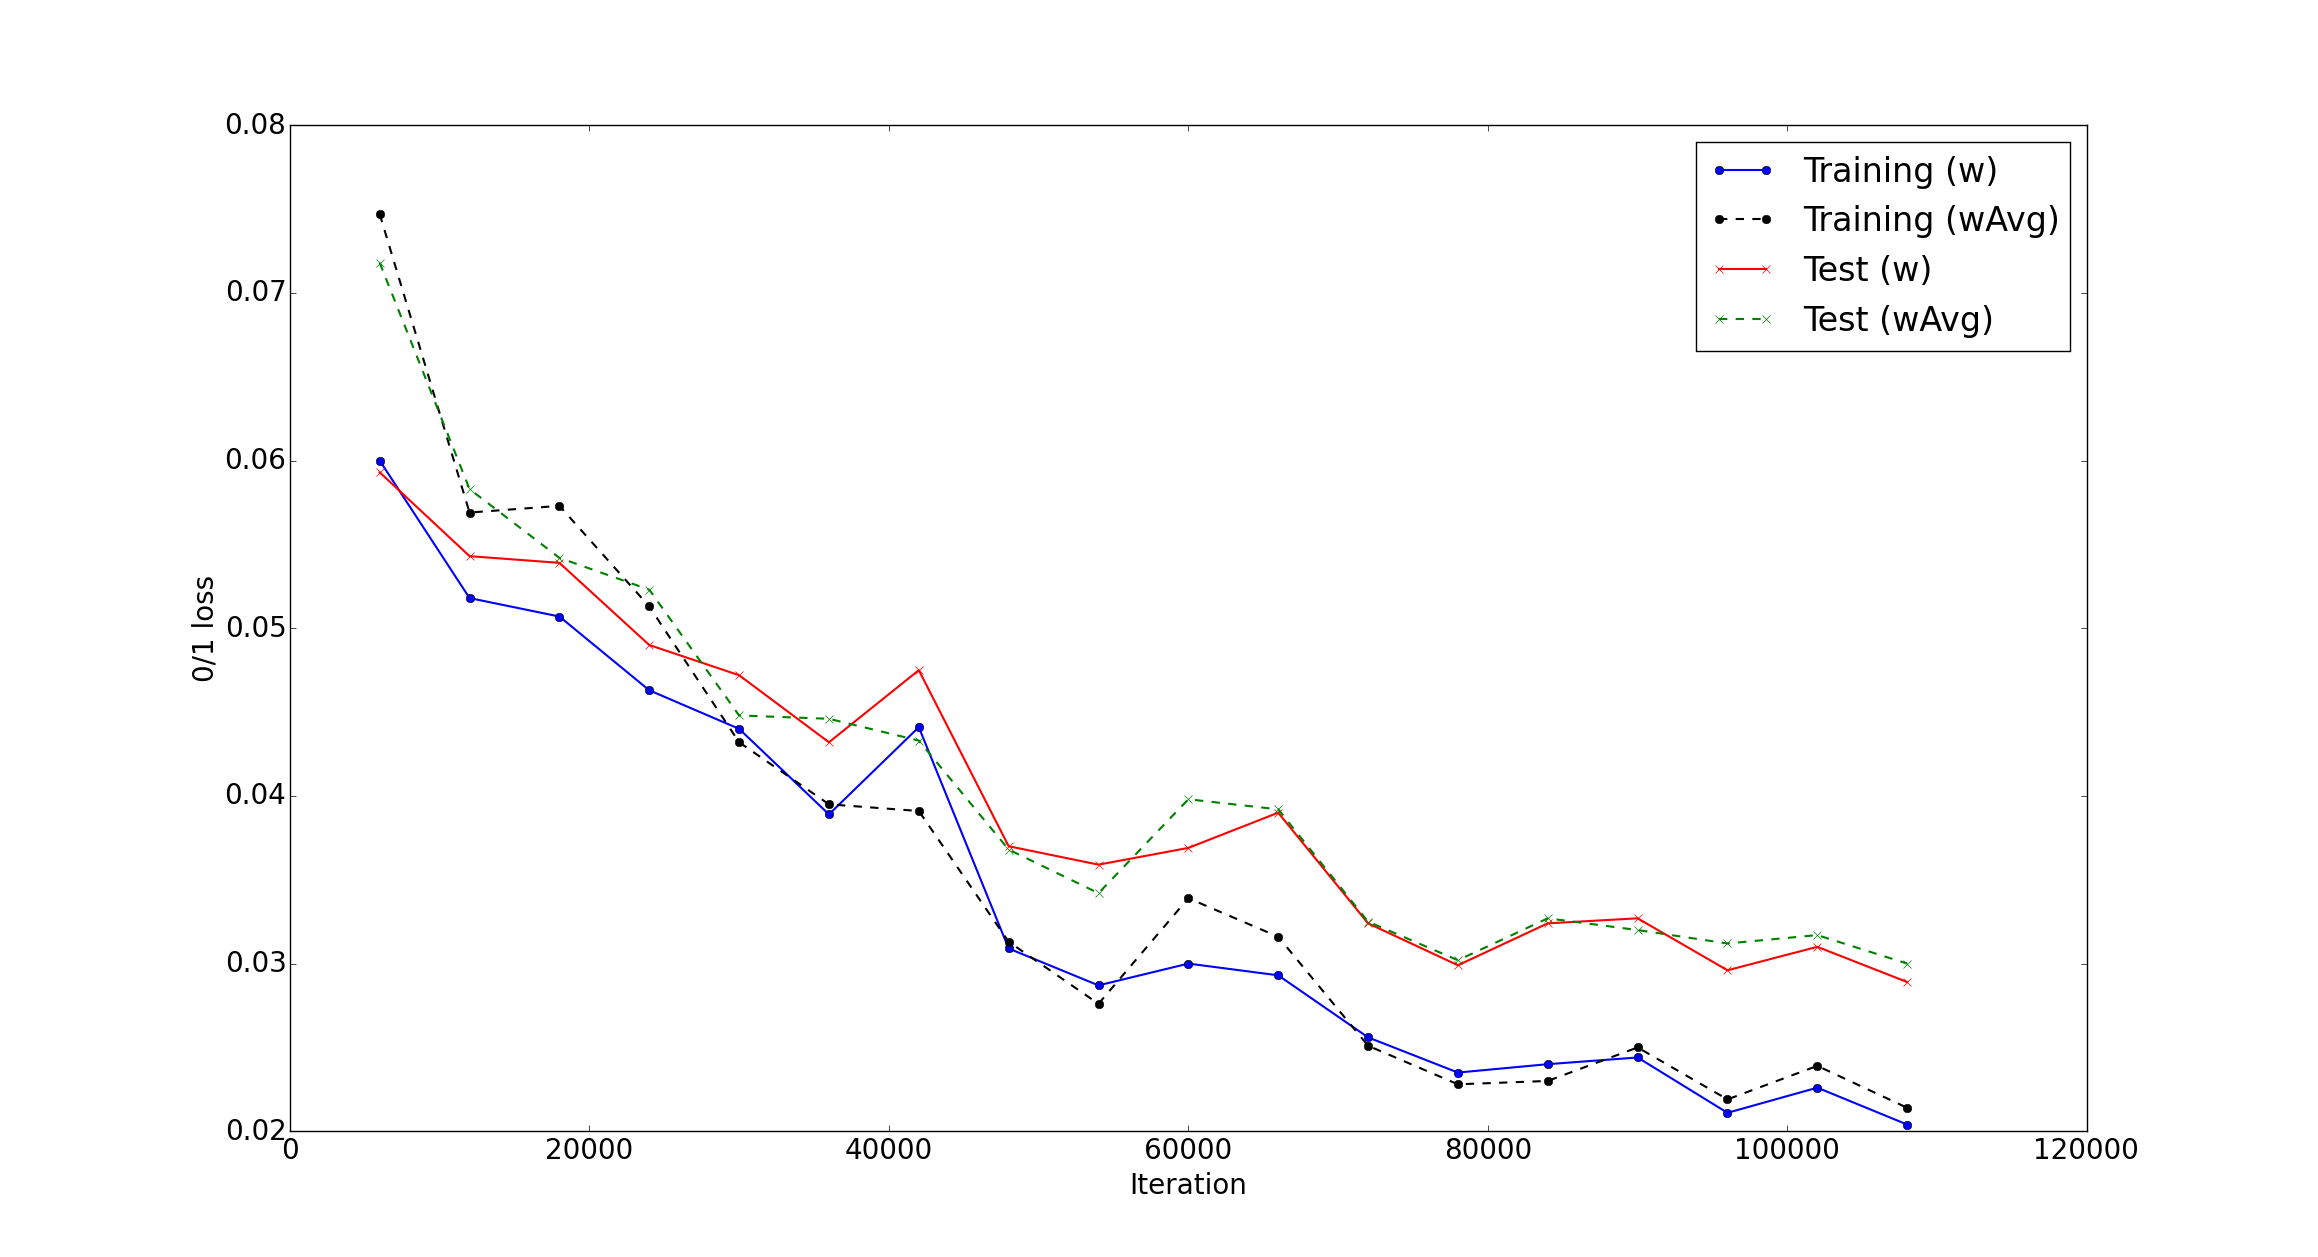
\includegraphics[width=.95\textwidth]{z1LossNNFeats18Epochs}
        \caption{The 0/1 loss of Stochastic gradient descent for the softmax classification problem applied to random neural net features of the projected MNIST dataset as a function of iteration, starting at iteration 0}
        \label{fig:z1LossNNFeats18Epochs}
    \end{figure}
    Figure \ref{fig:z1LossNNFeats18Epochs} is a visualization of the 0/1 loss for this problem, starting after an epoch has passed. Plotted are the 0/1 losses for the training and test data, with both the true weights and the epoch-averages.
    \item The final log and 0/1 losses on the training set were 0.15810703 and 0.0204, respectively. This 0/1 loss corresponds to 1734 missclassified images out of 60000.
    \item The final log and 0/1 losses on the test set were 0.25704783 and 0.0289, respectively. This 0/1 loss corresponds to 289 missclassifications out of 10000.
\end{enumerate}

% ---------------------------------

% Problem 3
\section{SVMs: Hinge loss and mistake bounds}
\begin{enumerate}
	\item To show that $\ell((x,y),w)=\max\{0,1-w\cdot x\}$ is convex with respect to $w$, we will need two observations. First, for any $a,k\in\R$ with $k\geq 0$, we have that
	\[
		\max\{0,ka\} = k\max\{0,a\}.
	\]
	In the case $ka<0$, both sides of the equality are 0. If $ka\geq 0$, then $a\geq0$ and the equality still holds. Next, for any $a,b\in\R$, we have
	\[
		\max\{0,a+b\}\leq \max\{0,a\}+\max\{0,b\}.
	\]
	If both $a$ and $b$ are negative, then the above is an equality. If exactly one of $a$ and $b$ is negative and $a+b\leq0$ then the inequality clearly holds. If both are nonnegative then it is also an equality.
	\vskip 0.1cm
	Recall that a function $f$ is convex if for any $t\in[0,1]$ and for any $x,y$ in its domain, $f(tx+(1-t)y)\leq tf(x)+(1-t)f(y)$. We will show that $\ell((x,y),w)$ has this property with respect to $w$. Let $w_1,w_2\in\R^d$ be arbitrary and let $t\in[0,1]$. Then $0\leq(1-t)\leq1$, and so
	\begin{align*}
		\ell\left((x,y),tw_1+(1-t)w_2\right) &= \max\{0,1-y(tw_1+(1-t)w_2)\cdot x\}\\
		&= \max\{0,1-tyw_1\cdot x-(1-t)yw_2\cdot x \}\\
		&= \max\{0,1+(t-t)-tyw_1\cdot x-(1-t)yw_2\cdot x \}\\
		&= \max\{0,[t-tyw_1\cdot x] + [(1-t)-(1-t)yw_2\cdot x] \}\\
		&\leq \max\{0,t-tyw_1\cdot x\}+\max\{(1-t)-(1-t)`yw_2\cdot x \}\\
		&= t\max\{0,1-yw_1\cdot x\}+(1-t)\max\{1-yw_2\cdot x \}\\
		&= t\ell((x,y),w_1)+(1-t)\ell((x,y),w_2).
	\end{align*}
	Therefore $\ell((x,y),w)$ is convex with respect to $w$.
	\item By its definition it is clear that $0\leq\ell((x,y),w)$. If $y_i=\mathrm{sgn}(w\cdot x_i)$ then $y_iw\cdot x_i\geq 0$, implying that $1- y_iw\cdot x_i\leq 1$. Hence $\ell((x_i,y_i),w)=\max\{0,1-y_iw\cdot x_i\}\leq 1$. Combining these bounds we get
	\[
		0\leq \ell((x_i,y_i),w)\leq 1
	\]
	for correctly classified points.
	\item Observe that if we misclassify a point (so that $y_i=-\mathrm{sgn}(w\cdot x_i)$) then $y_iw\cdot x_i\geq0$. Hence $\ell((x_i,y_i),w)\geq 1$ for misclassified points. Let $I\subset \{1,2,\dots,n\}$ be the indices corresponding to the data points which $w$ misclassifies. It follows that $|I|=M(w)$. By the previous part we know that for correct classifications the hinge loss is bounded between 0 and 1. Putting this all together we obtain
	\[
		M(w) = \sum_{i=1}^{M(w)}1 = \sum_{i\in I}1 \leq \sum_{i\in I}\ell((x_i,y_i),w)\leq\sum^n_{i=1}\ell((x_i,y_i),w)= \sum^n_{i=1}\max\{0,1-y_iw\cdot x_i\}.
	\]
	Dividing both sides by $n$ gives the desired result.
\end{enumerate}

% Problem 4
\section{Fitting an SVM classifier by hand}
We will use the equations
\begin{align}
	\bm{\hat w},\hat w_0 =\mathrm{argmin}\|w\|^2 \quad s.t. \label{eqn:1}\\
	y_1(w^T\phi(x_1)+w_0)\geq 1 \label{eqn:2}\\
	y_2(w^T\phi(x_2)+w_0)\geq 1. \label{eqn:3}
\end{align}
\begin{enumerate}
	\item The optimal vector $\bm{\hat w}$ is orthogonal to the decision boundary, which, in this case, should be the plane lying directly in the middle of $\phi(x_1) = (1,0,0)^T$ and $\phi(x_2)=(1,2,2)^T$. Hence $\bm{\hat w}$ is a normal vector for this plane and all normal vectors for this plane are proportional to $\phi(x_2)-\phi(x_1) = (0,2,2)^T$. Hence $\bm{\hat w} = \alpha (0,1,1)^T$ for some $\alpha\in\R$. In particular $(0,1,1)^T$ is parallel to $\bm{\hat w}$.
	\item Since the decision boundary is the plane in the middle of the two new features, the margin is simply half the distance between the two points $\phi(x_1)$ and $\phi(x_2)$. I.e. the margin is
	\[
		\frac12 \|\phi(x_2)-\phi(x_1)\| = \frac12 \|(0,2,2)^T\| = \frac12 (2\sqrt{2}) = \sqrt{2}.
	\]
	\item Since the margin is equal to $1/\|\bm{\hat w}\|$, we know that $\|\bm{\hat w}\|= 1 / \sqrt{2}$. From before, $\|\bm{\hat w}\| = \|\alpha(0,1,1)\| = \alpha\sqrt{2}$. Equating these two expressions, we see that $\alpha = \tfrac12$, so
	\[
		\bm{\hat w} = \frac12\bbm0\\1\\1\ebm = \bbm 0\\ 1/2 \\ 1/2 \ebm.
	\]
	\item Having determined $\bm{\hat w}$ we are now in a position to solve for $w_0$. Equation (\ref{eqn:1}) now simply states that we should choose $w_0$ to have minimal magnitude. Plugging into constraints (\ref{eqn:2}) and (\ref{eqn:3}), we get
	\begin{align*}
		y_1(w^T\phi(x_1)+w_0) &= -1[(0,1/2,1/2)\cdot(1,0,0)+w_0] &=~ -w_0 & \geq1 &\implies w_0\leq -1 \\
		y_2(w^T\phi(x_2)+w_0) &= 1[(0,1/2,1/2)\cdot(1,2,2)+w_0] &= 2+w_0 & \geq 1 &\implies w_0\geq -1.
	\end{align*}
	The only value for $w_0$ which satisfies both of these constraints is $w_0=-1$.
	\item Substituting in the values we found, we obtain
	\[
		f(x) = \hat w_0 + \bm{\hat w^T}\phi(x) = -1 + (0,1/2,1/2)\cdot(1,\sqrt{2}x,x^2) = -1 + \frac{\sqrt{2}}{2}x+\frac12x^2.
	\]
	\begin{figure}
        \centering
        \includegraphics[width=.85\textwidth]{discriminant}
        \caption{The discriminant function $f(x)$ (blue) and the two points in the dataset (red)} 
        \label{fig:discr}
    \end{figure}
    Figure \ref{fig:discr} shows a 2d plot of this discriminant function (generated in Mathematica). The blue curve is the graph of the function and the red points are the values of $f$ at the two data points. Note that $f$ evaluates to -1 and 1 at the two points.
\end{enumerate}


% Problem 5
\section{K-Means}
For this problem I chose to cluster on the 50-dimensional dataset. For the visualizations of the means I projected back up to the 784-dimensional space. It should also be noted that in order to improve numerical stability in the computation of the square reconstruction error, I first divided all the points in the dataset by the 2-norm of the largest magnitude entry. This preserves the geometry of the points, but alters the numerical value of the squared reconstruction error (but not its qualitative behavior). I made sure to rescale the means appropriately before projecting them back up to 784 dimensions.

\subsection{Run the algorithm}

\begin{enumerate}
	\item I initialized K-means in a naive way by simply selecting 16 random points from the data set to be the initial means. The code for this problem is contained in \texttt{hw3-5.py}.
	\begin{figure}
		\centering
	    	\includegraphics[width=0.7\textwidth]{kmeansReconErr16}
	    	\caption{Squared reconstruction error as a function of iteration number for 16 means}
	    	\label{fig:kmErr16}
	\end{figure}
	\begin{figure}
		\centering
	    	\includegraphics[width=0.85\textwidth]{kmeansClassAssign16}
	    	\caption{The number of data points assigned to each class using 16 means}
	    	\label{fig:kmAs16}
	\end{figure}
	\begin{figure}
		\centering
		\includegraphics[width=\textwidth]{kmeansMeans16}
		\caption{Visualizations of the 16 means, ordered (descending) from top-left to bottom-right by the number of data points assigned to them}
		\label{fig:kmVis16}
	\end{figure}

	\begin{enumerate}
		\item Figure \ref{fig:kmErr16} shows the squared reconstruction error as a function of iteration number of the K-means algorithm with 16 means. As I mentioned above, this is the squared reconstruction error for the rescaled projections of the data points onto the first 50 singular vectors.
		\item Figure \ref{fig:kmAs16} gives the numbers of data points assigned to each of the means in descending order. Along the x-axis are the labels associated with each mean.
		\item Figure \ref{fig:kmVis16} provides visualizations of the 16 means. The top left image corresponds to the mean with the most points assigned to it and the one in the bottom left to the mean with the least. The images are sorted in descending order in the same order as one would read text (from top to bottom, left to right).
	\end{enumerate}

	\item The means that output by the method do in fact look as if they each correspond to specific digits or averages of two similar looking digits. Since there are more than 10 possible classes, the means correspond to specific digits and digits that look similar to one another. Some digits can be drawn in multiple ways and have multiple means corresponding to each style. The mean with the most data points assigned to it looks to be somewhere between a 9 and a 7, so it is likely that some 9's and some 7's are placed in its cluster. There are two variations of 1 present, a vertical one and a somewhat tilted one. There are also means that look to be close to both 8's and 3's, 9's and 4's and 5's and 8's. This output is a good sanity check that K-means is doing what we think it should do for this dataset.

	\item I used the same initialization and rescaling procedures for 250 means as in the previous part of the problem.

	\begin{figure}
		\centering
	    	\includegraphics[width=0.7\textwidth]{kmeansReconErr250}
	    	\caption{Squared reconstruction error as a function of iteration number for 250 means}
	    	\label{fig:kmErr250}
	\end{figure}
	\begin{figure}
		\centering
	    	\includegraphics[width=0.85\textwidth]{kmeansClassAssign250}
	    	\caption{The number of data points assigned to each class using 250 means}
	    	\label{fig:kmAs250}
	\end{figure}

	\begin{figure}
		\centering
		\includegraphics[width=\textwidth]{kmeansMeans250}
		\caption{Visualizations of the 16 randomly selected means, ordered (descending) from top-left to bottom-right by the number of data points assigned to them}
		\label{fig:kmVis250}
	\end{figure}

	\begin{enumerate}
		\item Figure \ref{fig:kmErr250} shows the squared reconstruction error as a function of iteration number of the K-means algorithm with 250 means. As I mentioned above, this is the squared reconstruction error for the rescaled projections of the data points onto the first 50 singular vectors.
		\item Figure \ref{fig:kmAs250} gives the numbers of data points assigned to each of the means in descending order. Along the x-axis are the labels associated with each mean.
		\item Figure \ref{fig:kmVis250} provides visualizations of a random selection of 16 of the 250 means. The top left image corresponds to the mean with the most points assigned to it and the one in the bottom left to the mean with the least. The images are sorted in descending order in the same order as one would read text (from top to bottom, left to right).
	\end{enumerate}
\end{enumerate}

\subsection{Classification with K-means}
Since my initialization procedure is random, I get slightly different results each time I re-run K-means. Here I present losses which are representative of the typical losses.
\begin{enumerate}
	\item For $K=16$, my 0/1 losses for the training and test sets are 0.314 and 0.311, respectively.
	\item For $K=250$, my 0/1 losses for the training and test sets are 0.087 and 0.085, respectively.
\end{enumerate}


\end{document}

